\documentclass[aspectratio=169,11pt]{beamer}
\usetheme{default}
\setbeamertemplate{navigation symbols}{}
\setbeamertemplate{footline}{%
  \hfill\insertframenumber/\inserttotalframenumber\hspace*{4pt}\vspace{2pt}%
}
\usepackage{lmodern}
\usepackage[most]{tcolorbox}
\usepackage{listings}
\usepackage{tikz}
\usetikzlibrary{arrows.meta,positioning,shapes.geometric,fit,backgrounds}
\usepackage{booktabs}
\usepackage{hyperref}

\definecolor{lcgreen}{HTML}{2E7D32}
\definecolor{lcblue}{HTML}{1565C0}
\definecolor{lcorange}{HTML}{EF6C00}
\definecolor{lcred}{HTML}{C62828}
\definecolor{codebg}{HTML}{F5F5F5}
\definecolor{docgray}{gray}{0.55}

\newtcolorbox{conceptbox}[1][]{colback=yellow!20,colframe=yellow!60!black,title=#1,fonttitle=\bfseries,top=2pt,bottom=2pt,left=4pt,right=4pt}
\newtcolorbox{warningbox}[1][]{colback=red!15,colframe=red!60!black,title=#1,fonttitle=\bfseries,top=2pt,bottom=2pt,left=4pt,right=4pt}
\newtcolorbox{tipbox}[1][]{colback=green!10,colframe=green!50!black,title=#1,fonttitle=\bfseries,top=2pt,bottom=2pt,left=4pt,right=4pt}
\newtcolorbox{codebox}[1][]{colback=blue!10,colframe=blue!40!black,title=#1,fonttitle=\bfseries,top=2pt,bottom=2pt,left=4pt,right=4pt}

\lstset{
  basicstyle=\ttfamily\scriptsize,
  backgroundcolor=\color{codebg},
  breaklines=true,
  frame=single,
  rulecolor=\color{blue!40!black},
  keywordstyle=\color{lcblue}\bfseries,
  stringstyle=\color{lcgreen},
  commentstyle=\color{docgray}\itshape,
  language=Python,
  showstringspaces=false,
  tabsize=2,
  xleftmargin=2pt,
  xrightmargin=2pt,
  aboveskip=2pt,
  belowskip=2pt,
}

\newcommand{\docref}[1]{{\scriptsize\color{docgray}[Docs: #1]}}

\title{Section 07: Human-in-the-Loop}
\subtitle{Agents and Humans Collaborating Through Graph Interrupts}
\author{LangGraph v1.0.x (March 2026)}
\date{}

\begin{document}

\frame{\titlepage}

\begin{frame}{Mental Model: Why Human-in-the-Loop?}
  \begin{conceptbox}[The Big Picture]
    \setlength{\itemsep}{1pt}
    \begin{itemize}
      \item Agents make mistakes or take risky actions
      \item Humans provide \textbf{oversight}, \textbf{judgment}, \textbf{final approval}
      \item Interrupt graph, show human state, wait for decision
      \item Resume when human approves or edits
    \end{itemize}
  \end{conceptbox}
  \vspace{0.1cm}
  \begin{tipbox}[Essential for Production]
    HITL is critical for high-stakes decisions (financial, medical, legal).
  \end{tipbox}
\end{frame}

\begin{frame}{Breakpoints: The Two Interrupt Types}
  \begin{conceptbox}[interrupt\_before]
    \setlength{\itemsep}{1pt}
    \begin{itemize}
      \item Pauses \textbf{before} a node executes
      \item Human reviews state and inputs, then approves
      \item Example: block before calling ``delete\_database'' tool
    \end{itemize}
  \end{conceptbox}
  \vspace{0.1cm}
  \begin{conceptbox}[interrupt\_after]
    \setlength{\itemsep}{1pt}
    \begin{itemize}
      \item Pauses \textbf{after} a node executes
      \item Human sees output, can edit before next node
      \item Example: review agent's decision before proceeding
    \end{itemize}
  \end{conceptbox}
\end{frame}

\begin{frame}[fragile]{Setting Breakpoints: interrupt\_before}
  \begin{codebox}[Configure Interrupts at Compile Time]
    \begin{lstlisting}
graph = builder.compile(
  checkpointer=checkpointer,
  interrupt_before=["dangerous_tool_node"]
)
result = graph.invoke(
  {"messages": [HumanMessage("Delete old files")]},
  config={"configurable": {"thread_id": "123"}}
)
    \end{lstlisting}
  \end{codebox}
  \vspace{0.1cm}
  \begin{tipbox}[Breakpoint List]
    Pass list of node names. Graph pauses before executing those nodes.
  \end{tipbox}
\end{frame}

\begin{frame}[fragile]{Setting Breakpoints: interrupt\_after}
  \begin{codebox}[Pause After Node Execution]
    \begin{lstlisting}
graph = builder.compile(
  checkpointer=checkpointer,
  interrupt_after=["agent_node"]
)
result = graph.invoke(
  {"messages": [HumanMessage("Write email")]},
  config={"configurable": {"thread_id": "123"}}
)
    \end{lstlisting}
  \end{codebox}
  \vspace{0.1cm}
  \begin{tipbox}[Use Cases]
    Review draft outputs, approve decisions, edit state before proceeding.
  \end{tipbox}
\end{frame}

\begin{frame}[fragile]{How Interrupts Work}
  \begin{codebox}[Interrupt Flow]
    \begin{lstlisting}
config = {"configurable": {"thread_id": "conv_123"}}
try:
  result = graph.invoke(
    {"messages": [HumanMessage("Action")]},
    config=config
  )
except GraphInterrupt:
  state = graph.get_state(config)
  print(f"Paused at: {state.next}")
  print(f"State: {state.values}")
    \end{lstlisting}
  \end{codebox}
  \vspace{0.1cm}
  \begin{tipbox}[Async-Friendly]
    Interrupts work with both sync and async execution.
  \end{tipbox}
\end{frame}

\begin{frame}[fragile]{Resuming After Interrupt}
  \begin{codebox}[Resume with None Input]
    \begin{lstlisting}
config = {"configurable": {"thread_id": "conv_123"}}
state = graph.get_state(config)
print(f"Pending node: {state.next}")
human_approval = input("Approve? (y/n): ")
if human_approval == "y":
  result = graph.invoke(None, config=config)
  print(result)
    \end{lstlisting}
  \end{codebox}
  \vspace{0.1cm}
  \begin{tipbox}[Resume with None]
    \texttt{invoke(None, config=...)} continues from last checkpoint without new input.
  \end{tipbox}
\end{frame}

\begin{frame}[fragile]{Approval Patterns: Pre-Tool Execution}
  \begin{codebox}[Approve Tool Calls]
    \begin{lstlisting}
graph = builder.compile(
  checkpointer=checkpointer,
  interrupt_before=["tools"]
)
result = graph.invoke(input, config)
state = graph.get_state(config)
tool_calls = state.values["messages"][-1].tool_calls
for call in tool_calls:
  approved = human_approves(call)
  if not approved:
    graph.update_state(config, {"skip_tool": True})
result = graph.invoke(None, config)
    \end{lstlisting}
  \end{codebox}
  \vspace{0.1cm}
  \begin{tipbox}[Safety First]
    Block dangerous tool calls before execution.
  \end{tipbox}
\end{frame}

\begin{frame}[fragile]{Editing State Before Resuming}
  \begin{codebox}[Manual State Modification]
    \begin{lstlisting}
config = {"configurable": {"thread_id": "conv_123"}}
state = graph.get_state(config)
print(f"Current messages: {state.values['messages']}")
edited_messages = state.values["messages"]
edited_messages.append(
  HumanMessage("Correction: use this instead")
)
graph.update_state(config, {"messages": edited_messages})
result = graph.invoke(None, config)
    \end{lstlisting}
  \end{codebox}
  \vspace{0.1cm}
  \begin{tipbox}[Human Feedback Loop]
    Let humans correct mistakes in graph state mid-execution.
  \end{tipbox}
\end{frame}

\begin{frame}{The Command Primitive}
  \begin{conceptbox}[Command Types]
    \setlength{\itemsep}{1pt}
    \begin{itemize}
      \item \texttt{Command(resume=value)}: pass human input to graph
      \item \texttt{Command(goto=node\_name)}: jump to specific node
      \item \texttt{Command(resume=None)}: continue with no new input
    \end{itemize}
  \end{conceptbox}
  \vspace{0.1cm}
  \begin{tipbox}[Advanced Control]
    Commands enable precise control over graph execution flow.
  \end{tipbox}
\end{frame}

\begin{frame}[fragile]{Using Command(resume=value)}
  \begin{codebox}[Pass Human Input Back]
    \begin{lstlisting}
from langgraph.types import Command
state = graph.get_state(config)
human_decision = input("Approve? Yes/No: ")
if human_decision == "Yes":
  graph.update_state(
    config,
    Command(resume=HumanMessage("Approved"))
  )
result = graph.invoke(None, config)
    \end{lstlisting}
  \end{codebox}
  \vspace{0.1cm}
  \begin{tipbox}[User Feedback Integration]
    Commands let you inject human decisions back into graph state.
  \end{tipbox}
\end{frame}

\begin{frame}[fragile]{Using interrupt() Inside Nodes}
  \begin{codebox}[Inline Interrupts]
    \begin{lstlisting}
from langgraph.types import interrupt
def approval_node(state):
  decision = interrupt(
    f"Approve action: {state['action']}?"
  )
  if decision == "approve":
    return {"approved": True}
  else:
    return {"approved": False}
builder.add_node("approval", approval_node)
    \end{lstlisting}
  \end{codebox}
  \vspace{0.1cm}
  \begin{tipbox}[Dynamic Interrupts]
    Use \texttt{interrupt()} to pause mid-node, not just at node boundaries.
  \end{tipbox}
\end{frame}

\begin{frame}{TikZ Diagram: HITL Flow}
  \begin{center}
    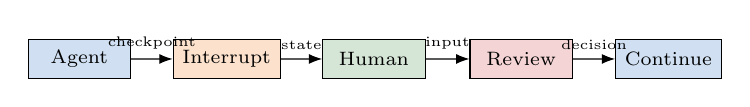
\begin{tikzpicture}[scale=0.85, every node/.style={font=\scriptsize}]
      \node[draw, rectangle, fill=lcblue!20, minimum width=1.3cm, minimum height=0.5cm] (agent) at (0, 2) {Agent};
      \node[draw, rectangle, fill=lcorange!20, minimum width=1.3cm, minimum height=0.5cm] (int) at (2.2, 2) {Interrupt};
      \node[draw, rectangle, fill=lcgreen!20, minimum width=1.3cm, minimum height=0.5cm] (human) at (4.4, 2) {Human};
      \node[draw, rectangle, fill=lcred!20, minimum width=1.3cm, minimum height=0.5cm] (decide) at (6.6, 2) {Review};
      \node[draw, rectangle, fill=lcblue!20, minimum width=1.3cm, minimum height=0.5cm] (cont) at (8.8, 2) {Continue};
      \draw[-Latex] (agent) -- (int) node[midway, above]{\tiny checkpoint};
      \draw[-Latex] (int) -- (human) node[midway, above]{\tiny state};
      \draw[-Latex] (human) -- (decide) node[midway, above]{\tiny input};
      \draw[-Latex] (decide) -- (cont) node[midway, above]{\tiny decision};
    \end{tikzpicture}
  \end{center}
  \vspace{0.1cm}
  \begin{tipbox}[Full Loop]
    Agent pauses, human reviews, returns decision. Loop continues or stops.
  \end{tipbox}
\end{frame}

\begin{frame}[fragile]{Multiple Breakpoints in One Graph}
  \begin{codebox}[Multi-Point Interrupts]
    \begin{lstlisting}
graph = builder.compile(
  checkpointer=checkpointer,
  interrupt_before=[
    "approve_decision",
    "execute_payment"
  ],
  interrupt_after=["draft_email"]
)
    \end{lstlisting}
  \end{codebox}
  \vspace{0.1cm}
  \begin{tipbox}[Flexible HITL]
    Different nodes can have different approval strategies.
  \end{tipbox}
\end{frame}

\begin{frame}{Dynamic Approval: Only High-Risk Actions}
  \begin{conceptbox}[Conditional Approval]
    \setlength{\itemsep}{1pt}
    \begin{itemize}
      \item Don't interrupt for every tool call
      \item Only approve high-risk: delete, transfer money, send emails
      \item Low-risk tools (search, read) execute automatically
    \end{itemize}
  \end{conceptbox}
  \vspace{0.1cm}
  \begin{tipbox}[User Experience]
    Minimize interruptions. Only pause when humans genuinely need to decide.
  \end{tipbox}
\end{frame}

\begin{frame}[fragile]{Dynamic Approval: Implementation}
  \begin{codebox}[Risk-Based Routing]
    \begin{lstlisting}
def should_interrupt(state):
  last_tool = state["messages"][-1].tool_calls[0]
  if last_tool["name"] in ["delete", "transfer", "send"]:
    return "approval_node"
  else:
    return "execute_tools"
builder.add_conditional_edges(
  "agent", should_interrupt,
  {"approval_node": "approval_node", ...}
)
    \end{lstlisting}
  \end{codebox}
  \vspace{0.1cm}
  \begin{tipbox}[Smart Filtering]
    Use conditional edges to route risky vs safe tools.
  \end{tipbox}
\end{frame}

\begin{frame}{Timeout and Fallback Patterns}
  \begin{conceptbox}[Timeout Strategy]
    \setlength{\itemsep}{1pt}
    \begin{itemize}
      \item If human doesn't respond in N seconds, what happens?
      \item Option 1: Continue with default (risky)
      \item Option 2: Fail gracefully (safe)
      \item Option 3: Escalate to manager
    \end{itemize}
  \end{conceptbox}
  \vspace{0.1cm}
  \begin{tipbox}[Design Decision]
    Default depends on your risk tolerance and business logic.
  \end{tipbox}
\end{frame}

\begin{frame}[fragile]{Timeout Implementation}
  \begin{codebox}[Async Timeout with asyncio]
    \begin{lstlisting}
import asyncio
async def wait_for_approval(state, timeout=30):
  try:
    decision = await asyncio.wait_for(
      human_approval_future,
      timeout=timeout
    )
    return {"approved": decision}
  except asyncio.TimeoutError:
    return {"approved": False, "reason": "timeout"}
    \end{lstlisting}
  \end{codebox}
  \vspace{0.1cm}
  \begin{tipbox}[Production Ready]
    Always include timeouts for interactive workflows.
  \end{tipbox}
\end{frame}

\begin{frame}{Common Pitfalls}
  \begin{warningbox}[No Checkpointer with HITL]
    \setlength{\itemsep}{1pt}
    \begin{itemize}
      \item Without checkpointer, state is lost when interrupt fires
      \item Solution: always use checkpointer with HITL
    \end{itemize}
  \end{warningbox}
  \vspace{0.1cm}
  \begin{warningbox}[Lost Interrupts]
    \setlength{\itemsep}{1pt}
    \begin{itemize}
      \item Catching exceptions without handling interrupts properly
      \item Solution: distinguish \texttt{GraphInterrupt} from other exceptions
    \end{itemize}
  \end{warningbox}
  \vspace{0.1cm}
  \begin{warningbox}[Poor UX]
    \setlength{\itemsep}{1pt}
    \begin{itemize}
      \item Too many interrupts frustrate users
      \item Solution: only interrupt for genuinely risky actions
    \end{itemize}
  \end{warningbox}
\end{frame}

\begin{frame}[fragile]{Summary: HITL Cheat Sheet}
  \begin{codebox}[Quick Reference]
    \begin{lstlisting}
graph = builder.compile(
  checkpointer=checkpointer,
  interrupt_before=["risky_node"]
)
result = graph.invoke(input, config)
state = graph.get_state(config)
if state.next:
  human_approves = input("OK? ")
  if human_approves:
    graph.invoke(None, config)
    \end{lstlisting}
  \end{codebox}
\end{frame}

\begin{frame}{Self-Check: Do You Understand?}
  \begin{enumerate}
    \setlength{\itemsep}{1pt}
    \item What's the difference between interrupt\_before and interrupt\_after?
    \item How do you resume after an interrupt?
    \item Why is a checkpointer essential for HITL?
    \item How do you edit state before resuming?
    \item What are Command types and when do you use them?
    \item How do you implement dynamic (risk-based) approval?
    \item What's a good timeout strategy for human approval?
  \end{enumerate}
\end{frame}

\end{document}
